\documentclass{standalone}
\usepackage[margin=1in,vmargin=1in]{geometry}
\usepackage{tikz}
\usepackage{graphicx}

%% neural network parameters
\newcommand\widthCirc{.5} % size of all circles
\newcommand\nodeSep{2} % node seperation along y axis
\newcommand\inputNodes{4} % input node count
\newcommand\hiddenNodes{5} % hidden node count
\newcommand\outputNodes{2} % output node count
\newcommand\inputSRow{1} % vertical off-set of input layer
\newcommand\hiddenSRow{6} % vertical off-set of hidden layer
\newcommand\outputSRow{3} % vertical off-set of output layer
\newcommand\numLayers{3} % number of layers ommiting output layer
\newcommand\twohiddenNodes{5} % second hidden layer node count
\newcommand\twohiddenSRow{0} % vertical off-set of second hidden layer

\newcommand\squareSize{0.6}
\newcommand\squareShift{3}
\newcommand\weightShift{2}

\newcommand\otdis{5 + \weightShift} % distance between layers

\begin{document}

\begin{centering}

  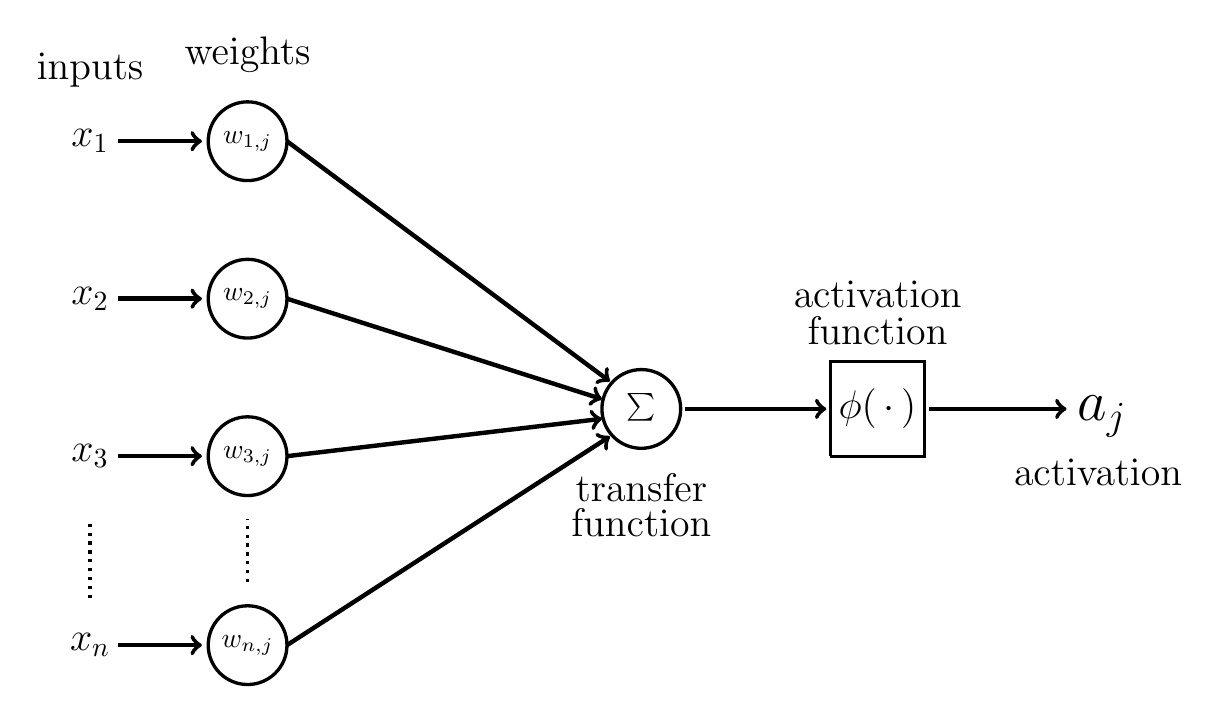
\begin{tikzpicture}[thick,scale=1, every node/.style={scale=1}]

    \node at (0,\inputSRow + \nodeSep * 4.65) {\Large{inputs}};
    \node at (\weightShift,\inputSRow + \nodeSep * 4.75) {\Large{weights}};

    \node at (0,\inputSRow + \nodeSep * 4.2) {\Large{$x_{1}$}};
    \node at (0,\inputSRow + \nodeSep * 3.2) {\Large{$x_{2}$}};
    \node at (0,\inputSRow + \nodeSep * 2.2) {\Large{$x_{3}$}};
    \node at (0,\inputSRow + \nodeSep * 1) {\Large{$x_{n}$}};

    \draw[ultra thick, ->] (0.35,\inputSRow+\nodeSep*1) -- (\weightShift-\widthCirc-0.08,\inputSRow+\nodeSep*1) node {};
    \draw[ultra thick, ->] (0.35,\inputSRow+\nodeSep*2.2) -- (\weightShift-\widthCirc-0.08,\inputSRow+\nodeSep*2.2) node {};
    \draw[ultra thick, ->] (0.35,\inputSRow+\nodeSep*3.2) -- (\weightShift-\widthCirc-0.08,\inputSRow+\nodeSep*3.2) node {};
    \draw[ultra thick, ->] (0.35,\inputSRow+\nodeSep*4.2) -- (\weightShift-\widthCirc-0.08,\inputSRow+\nodeSep*4.2) node {};


    \draw[very thick,black,dotted] (0,\inputSRow + \nodeSep * 1.3) -- (0,\inputSRow + \nodeSep * 1.8) {};


      \filldraw[color=black, fill=white, very thick](\weightShift,\inputSRow+\nodeSep*\inputNodes - \nodeSep*0.8 + \nodeSep) circle (\widthCirc) node {$w_{1,j}$};
      \filldraw[color=black, fill=white, very thick](\weightShift,\inputSRow+\nodeSep*\inputNodes - \nodeSep*1.8 + \nodeSep) circle (\widthCirc) node {$w_{2,j}$};
      \filldraw[color=black, fill=white, very thick](\weightShift,\inputSRow+\nodeSep*\inputNodes - \nodeSep*2.8 + \nodeSep) circle (\widthCirc) node {$w_{3,j}$};
      \filldraw[color=black, fill=white, very thick](\weightShift,\inputSRow+\nodeSep*\inputNodes - \nodeSep*4 + \nodeSep) circle (\widthCirc) node {$w_{n,j}$};

    \draw[very thick,black,dotted] (\weightShift,\inputSRow + \nodeSep * 1.4) -- (\weightShift,\inputSRow + \nodeSep * 1.8) {};
    \draw[ultra thick, ->] (\weightShift+\widthCirc,\inputSRow+\nodeSep*1) -- (\otdis-\widthCirc+.1,\hiddenSRow-0.35) node {};
    \draw[ultra thick, ->] (\weightShift+\widthCirc,\inputSRow+\nodeSep*2.2) -- (\otdis-\widthCirc,\hiddenSRow-.125) node {};
    \draw[ultra thick, ->] (\weightShift+\widthCirc,\inputSRow+\nodeSep*3.2) -- (\otdis-\widthCirc,\hiddenSRow+0.125) node {};
    \draw[ultra thick, ->] (\weightShift+\widthCirc,\inputSRow+\nodeSep*4.2) -- (\otdis-\widthCirc+.1,\hiddenSRow+0.35) node {};

    \filldraw[color=black, fill=white, very thick](\otdis,\hiddenSRow) circle (\widthCirc) node {\Huge{$\mathbf{\sum}$}};
    \node at (\otdis,\hiddenSRow-1) {\Large{transfer}};
    \node at (\otdis,\hiddenSRow-1.45) {\Large{function}};

    \draw[ultra thick, ->] (\otdis+\widthCirc+0.05,\hiddenSRow) -- (\otdis+\squareShift-\squareSize-0.05,\hiddenSRow) node {};

    \filldraw[color=black, fill=white, very thick] (\otdis+\squareShift-\squareSize,\hiddenSRow-\squareSize) -- (\otdis+\squareShift+\squareSize,\hiddenSRow-\squareSize) -- (\otdis+\squareShift+\squareSize,\hiddenSRow+\squareSize) -- (\otdis+\squareShift-\squareSize,\hiddenSRow+\squareSize) -- (\otdis+\squareShift-\squareSize,\hiddenSRow-\squareSize);

    \node at (\otdis+\squareShift,\hiddenSRow) {\Large{$\phi(\,\cdotp)$}};
    \node at (\otdis+\squareShift,\hiddenSRow+1.45) {\Large{activation}};
    \node at (\otdis+\squareShift,\hiddenSRow+1) {\Large{function}};

    \draw[ultra thick, ->] (\otdis+\squareShift+\squareSize+0.05,\hiddenSRow) -- (\otdis+\squareShift+\squareSize + 1.8,\hiddenSRow) node {};

    \node at (\otdis+\squareShift+\squareSize + 2.25,\hiddenSRow-.1) {\huge{$a_{j}$}};
    \node at (\otdis+\squareShift+\squareSize + 2.2,\hiddenSRow-0.8) {\Large{activation}};

  \end{tikzpicture}
\end{centering}

\end{document}
